\section{Technologien}
\label{sec:technology}
Im Verlauf dieser Sektion werden die Technologien und deren Verwendungszweck
kurz erläutert.

\subsection{Blattwerkzeug}
\label{sec:blattwerkzeug}

\begin{figure}
	
\includegraphics[scale=0.4]{graphics/blattwerkzeug.png}
\end{figure}


Blattwerkzeug ist ein quelloffenes Projekt, dass Informatik-Interessierten das Programmieren von \gls{HTML} Grundgerüsten und SQL Statements per \enquote{drag and drop} näher bringen kann. Dabei versteckt Blattwerkzeug die Syntax nicht vor dem Nutzer, sondern gibt ihm die Möglichkeit diesen gleich mit einzusehen. Dennoch ist es dem Nutzer einfach gemacht, mit visuellen Elementen teile der Informatik kennen zu lernen.

Dabei hat es sich Blattwerkzeug vor allem als Aufgabe gemacht an Schulen aufzutreten. Mit Blattwerkzeug wird Lehrern ein Werkzeug in die Hand gelegt, mit dem der Informatik Unterricht einfacher und informativer gestaltet werden kann. Somit wird der veraltete und doch sehr Office-lastige Informatik Unterricht komplett erneuert und interessanter gestaltet werden\todo{Zuviel: BlattWerkzeug ist ein Zusatz, keine Ersetzung}.

\subsection{Passwort Hashing}
\label{sec:password_hashing}

Sobald eine Software mit Nutzerdaten geführt wird, ergibt sich das Problem des Speicherns der Passwörter der jeweiligen Nutzer.
Denn sollten die Daten der Nutzer im Klartext in der Datenbank gespeichert werden und ein Angreifer erlangt Zugriff auf die Datenbank, so ist es für ihn ein leichtes weitere Konten der Nutzer zu infiltrieren. Der Grund dafür sind die anwendungsübergreifenden, vom Nutzer grö{\ss}tenteils identischen, Passwörter.

\todo[inline]{Nicht nur Super-GAU für eigene Seite, sondern auch für Nutzer auf anderen Seiten. Konkretes Beispiel ergänzen (Liesschen Müller ist mit ihrer EMail
  \enquote{lieeschen@müller.de} und dem Passwort \enquote{Milch} bei \enquote{Milchkanne.de} registriert, ...}

An diesem Punkt kommt das Hashen von Passwörtern zum Einsatz. Passwort Hashing soll dem Nutzer Sicherheit gewährleisten und es einem Angreifer nicht möglich machen mit erlangten Daten weitere Konten der Nutzer zu infiltrieren. Dabei wird aus einem Passwort ein Hash generiert. Dieser Hash macht es einem unmöglich, das Passwort wiederherzustellen. Jedoch ergibt sich bei gleicher Eingabe, der gleiche Hash. Um ein gehashtes Passwort zu erhalten, muss ein Hashing Algorithmus auf das jeweilige Klartext Passwort angewendet werden.

Mittlerweile gibt es eine vielzahl an Hashfunktionen, von denen manche als nicht mehr sicher gelten. Der Grund dafür sind Rainbowtables in denen Hashes mit dazugehörigem Klartext Passwort (Abbildung \ref{fig:unhashed_table}) stehen. Das Nutzen einer nicht sicheren Hashfunktion stellt ein Sicherheitsrisiko dar, da die Möglichkeit besteht, das gehashte Passwort mit einer Rainbowtable (Abbildung \ref{fig:rainbowtable}) abzugleichen und dabei das jeweilige Klartext Passwort zu erhalten. Aus diesem Grund werden MD5 (Abbildung \ref{fig:md5_hashed_table}) und SHA zwei der bekanntesten Hashfunktionen, seit geraumer Zeit nicht mehr zum Passwort hashen verwendet werden. Ein Beispiel für eine derzeitig nutzbare Hashfunktion ist bcrypt. Bcrypt bietet den Vorteil des Integrierten Saltings. (Abbildung \ref{fig:salted_table})

\begin{figure}
	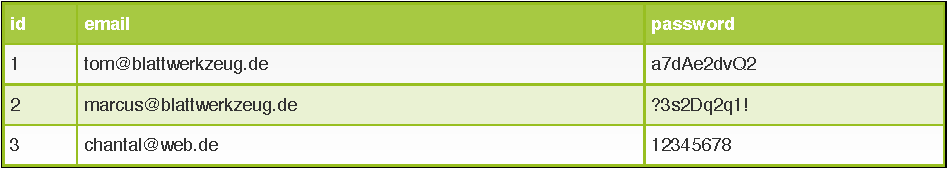
\includegraphics[width=\textwidth]{graphics/unhashed_table.pdf}
	\caption{Tabelle mit ungehashten Passwörtern}
	\label{fig:unhashed_table}
\end{figure}

\begin{figure}
	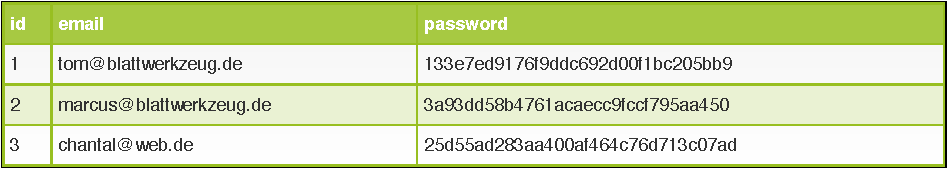
\includegraphics[width=\textwidth]{graphics/md5_table.pdf}
	\caption{Tabelle mit MD5 gehashten Passwörtern}
	\label{fig:md5_hashed_table}
\end{figure}

\begin{figure}
	\includegraphics[width=\textwidth]{graphics/salted_table.pdf}
	\caption{Tabelle mit Salting Hashes}
	\label{fig:salted_table}
\end{figure}

\begin{figure}
	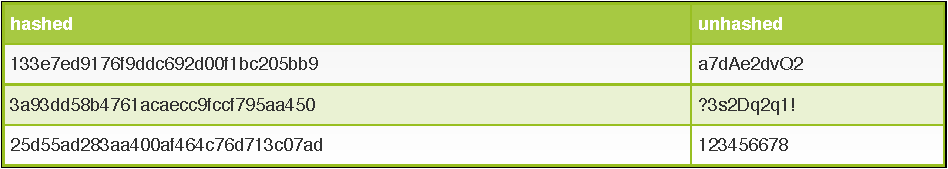
\includegraphics[width=\textwidth]{graphics/rainbowtable.pdf}
	\caption{Beispiel einer Rainbowtable.}
	\label{fig:rainbowtable}
\end{figure}

 Salts (Abbildung ~\ref{fig:salted-hash}) sind zufällig generierte Zeichenketten, die dem Klartext-Passwort hinzugefügt werden. Der zusammengesetzte String wird mittels Hashfunktion verschlüsselt.

\begin{figure}
	\centering
	\includegraphics[width=.89\textwidth]{graphics/salting.pdf}
	\caption{Hashfunktion auf Klartext und Salt angewandt.}
	\label{fig:salted-hash}
\end{figure}

\subsection{Sessions}
\label{sec: sessions}

Das \gls{HTTP} ist ein zustandsloses Protokoll, dass sich keine Informationen der jeweiligen Aufrufe zwischenspeichert. Dies ist aber unpraktisch, wenn Daten eines Benutzer kurzeitig gespeichert werden sollen. \todo{Zustandslos praktisch} Ein Verwendungszweck wäre beispielsweise der Warenkorb, da dieser nur temporär vorhanden sein soll. Genau dieses Problem kann mit der Session gelöst werden\todo{Warum lösen Cookies das Problem nicht?}.

Die Session ist eine serverseitige Daten-Speichermöglichkeit. Dabei wird bei der Anfrage von einem Client an den Server ohne Session-ID eine Session und Session-ID erstellt. Diese Session-ID wird bei der Antwort des Servers mit an den Client ausgeliefert. Ab diesem Punkt wird bei jeder Anfrage vom Client an den Server die Session-ID mit gesendet. Dies kann über einen Cookie oder über die \gls{URI} erfolgen. Aufgrund dessen kann der Server dem Client Daten aus der jeweiligen Session zur Verfügung stellen.

IMAGE

\subsection{JSON Web Token}
\label{sec: jwt}
\enquote{\gls{JWT} sind auf \gls{JSON} basierende \gls{RFC} 7519 genormte Access-Token.} \gls{RFC} ist eine Sammlung aus Dokumenten, in denen das Verhalten der Technologien des Internets beschrieben ist. Einige davon gehören zum Standard und werden somit in den meisten Fällen vorausgesetzt. In speziellen Fällen möchte beispielsweise ein Unternehmen eigene Protokolle verwenden, die nicht zum Standard gehören.

Diese Tokens werden zur eindeutigen Identifizierung von Nutzern verwendet und können die Session ersetzen. Dabei ist es bei einem \gls{JWT} nicht vonnöten die Daten auf dem Server zu speichern. Dies hat zur Folge, dass die Pflege des Speichers an diesem Punkt entfällt. Jedoch haben \gls{JWT}s einen gro{\ss}en Nachteil, denn sobald der Server einen \gls{JWT} ausgestellt hat, ist dieser bis zum Ablauf des Tokens gültig. Das hei{\ss}t, sollte ein Server die Berechtigung eines Nutzers nach Ausstellung eines \gls{JWT} ändern, ist diese Änderung erst bei erneutem Erstellen eines \gls{JWT} gültig.

Ein \gls{JWT} besteht aus Header, Payload und Signatur. Dabei ist der Header und die Payload jeweils ein \gls{JSON} Objekt.

\subsubsection{Header}
\label{sec: jwt_header}

\begin{description}
	\leftskip=1em
	\item[typ] Der typ Claim beschreibt den \gls{MIME} des \gls{JWT}, dieser wiederum teilt dem Client oder Server mit, um welche Art von Medium an Daten es sich handelt. Der Standardwert dieses Claims beläuft sich auf \enquote{JWT}, übersetzt \enquote{application/jwt}.
	\item[alg] Der alg Claim beschreibt die Verschlüsselungsmethode. Ein Beispiel ist \gls{HMAC} mit \gls{SHA256}, HS256 abgekürzt.
\end{description}

\begin{figure}[h]
	\centering
	\includegraphics[width=\textwidth]{graphics/jwt-header.png}
	\caption{Beispiel eines \gls{JWT} Headers }
	\label{fig:jwt-header}
\end{figure}

\subsubsection{Payload}
\label{sec: jwt-payload}

Die Payload beinhalteten Schlüssel-Wert Paare werden Claims genannt. Dabei handelt es sich um ein JSON Objekt, bei dem bestimmte Schlüssel des Objektes bereits reserviert sind. Diese nennen sich registrierte Claims. Au{\ss}erdem gibt es öffentliche und private Claims. Hierbei wird zwischen öffentlichen und privaten differenziert.

\noindent
\textbf{Beispiel registrierter Claims}

\begin{description}
	\leftskip=1em
	\item[iss]
	Der iss Claim steht für den Austeller des Tokens, beispielsweise eine Domain.
	\item[exp] Der exp Claim kennzeichnet den \gls{JWT} mit einem Ablaufdatum.
\end{description}

\noindent
\textbf{Öffentliche Claims}

Öffentliche Claims sind zusätzlich zum Standard nutzbar und ihre Namen sollten semantisch dem dazugehörigen Wert entsprechen. Au{\ss}erdem sollten die Namen der Claims Netzwerkübergreifend verständlich sein (Listing \ref{lst:public_claim}).

\noindent
\textbf{Private Claims}

Private Claims werden nur innerhalb eines Netzwerkes verwendet. Aus diesem Grund gibt es keine implizite Beschränkung in der Namensgebung (Listing \ref{lst:private_claim}).

\begin{minipage}{\linewidth}
	\lstinputlisting[label={lst:public_claim}, language=JSON, caption=Beispiel eines Öffentlichen Claims, captionpos=b]{snippets/public_claim.json}

	\lstinputlisting[label={lst:private_claim}, language=JSON, caption=Beispiel eines Privaten Claims, captionpos=b]{snippets/private_claim.json}
\end{minipage}

\subsubsection{Signatur}
\label{sec: jwt_signature}

Um die Signatur zu erhalten muss, die Payload und der Header Base64 kodiert werden. Au{\ss}erdem müssen diese beiden kodierten Zeichenfolgen mit einem Punkt als Trennzeichen verknüpft werden. Darauffolgend wird eine Hashfunktion auf das jeweilige Ergebnis mit zusätzlich sicherer Zeichenfolge als Parameter angewandt. Da diese sichere Zeichenfolge, auch Private Key genannt, nur auf dem Server hinterlegt ist, ist es dem Client zwar möglich den \gls{JWT} zu verändern, ihn jedoch mit korrekter Signatur zu versehen nicht.

\subsubsection{Zusammengesetzes Token}
\label{sec: jwt_result}
Schlussendlich ergibt sich der \gls{JWT} aus kodiertem Header, kodierten Payload und der Signatur. Dabei steht der Header am Anfang (Abbildung \ref{fig:jwt-encoded}, rot gekennzeichnet). Darauffolgend mit einem Punkt getrennt die Payload und zum Schluss die Signatur, ebenfalls mit einem Punkt getrennt.

\begin{figure}[h]
	\centering
	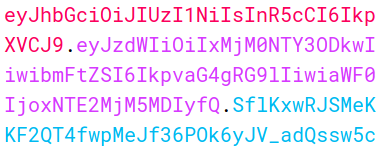
\includegraphics[width=\linewidth]{graphics/jwt-encoded.png}
	\caption{Beispiel eines kodierten \gls{JWT} }
	\label{fig:jwt-encoded}
\end{figure}

\subsection{Ruby on Rails}
\label{sec: rails}
Ruby on Rails ist ein quelloffenes Webframework für die Programmiersprache Ruby. Das Webframework nutzt das \gls{MVC} Muster und stellt bereits ein sehr umfangreiches \gls{CLI} zur Verfügung. Mittels des generate Werkzeugs kann beispielsweise Model, View und Controller erstellt werden. Jeder dieser Komponenten wird automatisch in die erstellte Rails Anwendung eingebunden. Au{/ss}erdem stellt Rails eine umfangreiche Test-Architektur und einen Service zum Versenden von Mails zur Verfügung. Dabei kann der Inhalt der E-Mail im Textformat oder als \gls{HTML} versendet werden. Einer der wesentlichen Vorteile von Ruby on Rails ist jedoch die Datenbankanbindung. Hierbei bietet Rails einen nachhaltigen und rücksichtsvollen Umgang mit der Datenbank, zum Beispiel die Migrationen. Migrationen erlauben, die Datenbank, ohne explizite SQL-Statements, zu verändern. Zusätzlich erleichtern Migrationen die Implementierung einer Datenbankstruktur auf einem anderen System.

\subsubsection{Routen}
\label{sec: routen}
Die Routen in Rails verweisen auf einen Controller und auf eine Funktion innerhalb des Controllers. Dabei wird die Route meistens mit der Anfragemethode eingeleitet, beispielsweise \enquote{get}. Routen können in sogenannte \enquote{scopes} (Listing \ref{lst:routes_scopes}) unterteilt werden. Somit ist es nicht vonnöten bei einer verschachtelten \gls{URI} redundant zu werden (Listung \ref{lst:routes_redundant}).

\begin{minipage}{\linewidth}
	\lstinputlisting[language=Ruby, style=CodeView, caption=Beispiel einiger redundanter Routen, captionpos=b, label={lst:routes_redundant}]{snippets/routes_redundant.rb}
\end{minipage}

\begin{minipage}{\linewidth}
	\lstinputlisting[language=Ruby, style=CodeView, caption=Beispiel einiger Routen mit scope, captionpos=b, label={lst:routes_scopes}]{snippets/routes.rb}
\end{minipage}

\subsubsection{Controller}
\label{sec: rails_controller}
Der Controller dient hierbei zur Kapselung von bestimmten Prozessen. Jede Route verweist in irgendeiner Weise auf eine Controller Funktion. In der jeweiligen Controller Funktion wird dann meistens mit einem Model interagiert. Es wird beispielsweise eine Benutzerberechtigung abgefragt und individuell auf die Berechtigung reagiert. Um auf die jeweilige Berechtigung zu reagieren, gibt es mehrere Möglichkeiten. Eine der Möglichkeiten wäre, direkt ein View Template auf dem Server zu rendern und an den Client auszuliefern. Eine andere Möglichkeit wäre ein \gls{JSON} Objekt zurück zu geben und darauf mit dem Client zu agieren.

\subsubsection{Model}
\label{sec: rails_model}
Das Model in Rails stellt jeweils eine Datenbanktabelle dar. Die Attribute des Models sind die entsprechenden Spalten der Datenbanktabelle. Jeweilige Datenbankeinträge, die über das Model erstellt werden, können mittels Validatoren auf ihre Gültigkeit geprüft werden. Diese Validatoren werden innerhalb des Models festgelegt und auf ein Attribut des Models zugewiesen. Rails bietet dabei bereits verfügbare Validatoren, zum Beispiel \enquote{presence: true}. Dieser Validator sorgt für das Vorhandensein eines Wertes ungleich \textit{nil}. Jedes Model kann zusätzliche Funktionen beinhalten, die direkt auf den jeweiligen Datenbankeintrag angewandt werden können. Ebenso bietet Rails die Möglichkeit die Beziehungen zwischen Datenbanktabellen direkt in den Modellen festzulegen.

\subsubsection{View}
\label{sec: rails_view}
Die View stellt in Rails die Möglichkeit \gls{HTML} Template auf dem Server zu rendern. Dabei kann bei dem Rendern das \gls{HTML} Template dynamisch verändert werden. Da diese Komponente während dieser Thesis keine Rolle gespielt hat, wird diese nicht weiter erläutert.

\subsubsection{Zusammenfassung}
\label{sec: rails_resuemee}
Letzendlich wird über die Route auf den jeweiligen Controller zugegriffen. Dieser fragt in den meisten Fällen nach einem bestimmten Eintrag eines Models. Darauffolgend wird mit dem Ergebnis der Anfrage interagiert. Es werden Veränderungen oder Abfragen bestimmter Daten getätigt. Danach wird ein Ergebnis dem Client ausgeliefert.

\begin{figure}[h]
	\includegraphics[width=\textwidth]{graphics/rails-mvc.pdf}
	\caption{Ablauf zwischen Client, Server, Route, Controller und Model}
	\label{fig:rails-mvc}
\end{figure}

\subsection{Angular}
\label{sec: angular}
Angular ist ein TypeScript basiertes Front-End Webframework, dass in vielen Fällen für \gls{SPA} verwendet wird. \gls{SPA}s laden ihren Inhalt lediglich in ein einziges \gls{HTML} Dokument. Der Inhalt dieses \gls{HTML} Dokumentes wird dynamisch, von beispielsweise einem Framework wie Angular, verändert. Der wesentliche Vorteil von Angular sind die klaren Entwurfsmuster. Jede Komponente in Angular hat im wesentlichen die gleiche Struktur. Dies hat zur Folge, dass Angular eine sehr gute Codekonsistenz bietet.


\subsubsection{Component}
\label{sec: ang-component}
Komponenten in Angular bieten die Möglichkeit \gls{HTML}, \gls{CSS} und TypeScript zu kapseln. Das bedeutet, dass jede Komponente unabhängig von einer anderen Komponente arbeiten kann.

\subsubsection{Services}
\label{sec: ang-service}
Zur Kommunikation mit einem Server und/oder zum Datenaustausch zwischen unterschiedlichen Komponenten wird meistens ein Service verwendet. Bei einem Datenaustausch zwischen Eltern- und Kind-Komponente ist es jedoch einfacher dies mittels der Kind-Komponente durchzuführen. Services werden bei dem Laden der Module instanziiert und dem Konstruktor der Komponente als instanziiertes Objekt übergeben.

\subsubsection{Module}
\label{sec: ang-modul}
Zusätzlich bietet Angular auch die Möglichkeit eigene Module zu erstellen in denen dann als Beispiel Services und Komponenten zusätzlich abgekapselt werden können. Ein Vorteil von Angular gegenüber anderen JavaScript Frameworks sind die bereits von Angular mitgelieferten Module, beispielsweise das Routing- oder das HTTP-Modul. Das Routing-Modul wird für jegliche Navigation auf der Anwendung genutzt. Das \gls{HTTP}-Modul hingegen bietet die Möglichkeit mittels jeglicher Anfragemethoden mit dem Server zu kommunizieren.

\subsection{oAuth2}
\label{sec: oauth2}
\gls{oAuth2} ist ein offenes \gls{RFC} 6749 Protokoll, welches verwendet wird, um eine Authentifizierung einer Anwendung mittels Drittanbieter zu ermöglichen. Hierbei wird der Nutzer zuerst auf die jeweilige Seite des Drittanbieters weitergeleitet. Dort muss der Nutzer sich authentifizieren und den Zugriff auf die Daten seines Kontos bestätigen. Nachdem der Zugriff auf die Daten bestätigt wurde, erhält die jeweilige Anwendung von dem Drittanbieter einen Autorisierungstoken. Dieser Autorisierungstoken wird darauffolgend von der Anwendung genutzt, um einen Zugriffstoken von dem Drittanbieter zu erhalten. Dieser ermöglicht am Ende den Zugriff auf die spezifischen Nutzerdaten des Drittanbieters. (Abbildung ~\ref{fig:oauth2})

In Blattwerkzeug wird genau dieser umfangreiche Vorgang von Omniauth übernommen. Aus diesem Grund wird oAuth2 in dieser Thesis nicht weiter erläutert.

\begin{figure}[h]
	\centering
	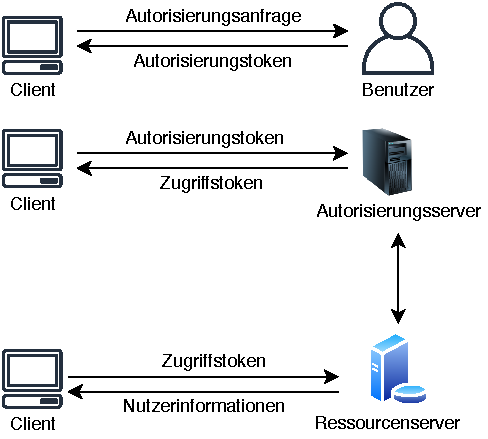
\includegraphics[width=.55\textwidth]{graphics/oauth2.pdf}
	\caption{oAuth2 verfahren}
	\label{fig:oauth2}
\end{figure}